Im Folgenden werden Tabellen und Abbildungen der Mediennutzung dargestellt. 

\begin{figure}[htp]
\caption{Medien \& Mediennutzung}\label{fig:AppMedienMediennutzung}
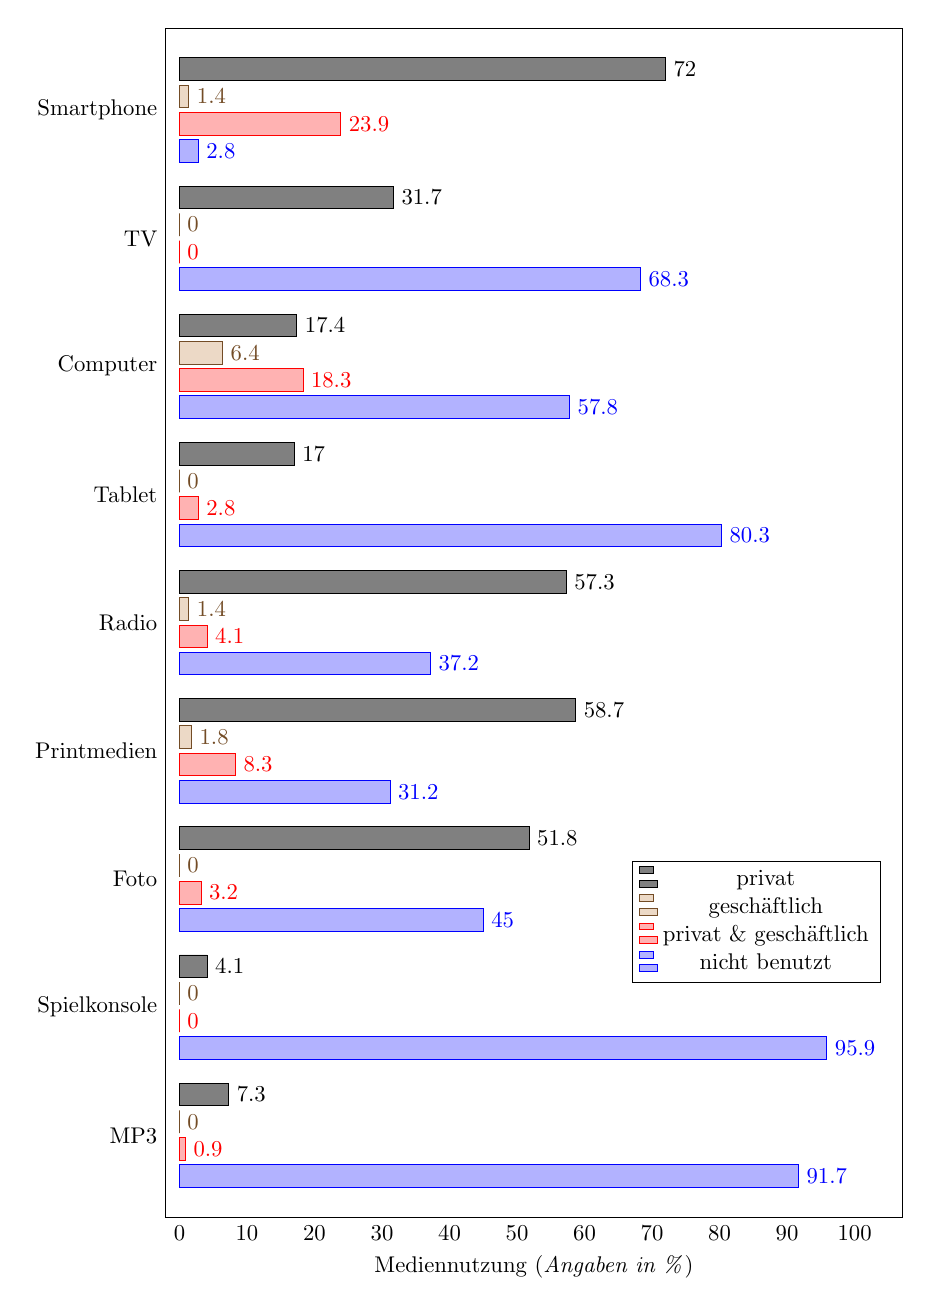
\begin{tikzpicture}[scale=0.82, auto]
  \begin{axis}[
    xbar,
    %y axis line style = { opacity = 0 },
    %axis x line       = none,
    tickwidth         = 0pt,
    xmin              = 0,
    xmax              = 105,
    enlarge y limits  = 0.08,
    enlarge x limits  = 0.02,
    reverse legend,
    %/legend pos=south east,
    legend style={at={(0.97,0.3)}},
    ytick             = data,
    xlabel            = {Mediennutzung (\textit{Angaben in \%})},
    height            = 20cm,
    width             = 13cm,
    symbolic y coords = {MP3, Spielkonsole, Foto, Printmedien, Radio, Tablet, Computer, TV, Smartphone},
    nodes near coords,
    nodes near coords align={horizontal},
  ]
  %nicht benutzt
  \addplot coordinates { (2.8,Smartphone)(68.3,TV)(57.8,Computer)(80.3,Tablet)(37.2,Radio)(31.2,Printmedien)(45,Foto)(95.9,Spielkonsole)(91.7,MP3)};
  %privat und geschäftlich
  \addplot coordinates { (23.9,Smartphone)(0,TV)(18.3,Computer)(2.8,Tablet)(4.1,Radio)(8.3,Printmedien)(3.2,Foto)(0,Spielkonsole)(0.9,MP3)};
  %geschäftlich
  \addplot coordinates { (1.4,Smartphone)(0,TV)(6.4,Computer)(0,Tablet)(1.4,Radio)(1.8,Printmedien)(0,Foto)(0,Spielkonsole)(0,MP3)};
  %privat
  \addplot coordinates { (72,Smartphone)(31.7,TV)(17.4,Computer)(17,Tablet)(57.3,Radio)(58.7,Printmedien)(51.8,Foto)(4.1,Spielkonsole)(7.3,MP3)};
  
  \legend{nicht benutzt, privat \& geschäftlich, geschäftlich, privat}
  \end{axis}
\end{tikzpicture}
\end{figure}

\begin{figure}[htp]
\caption{Medientätigkeit}\label{fig:AppMedientätigkeit}
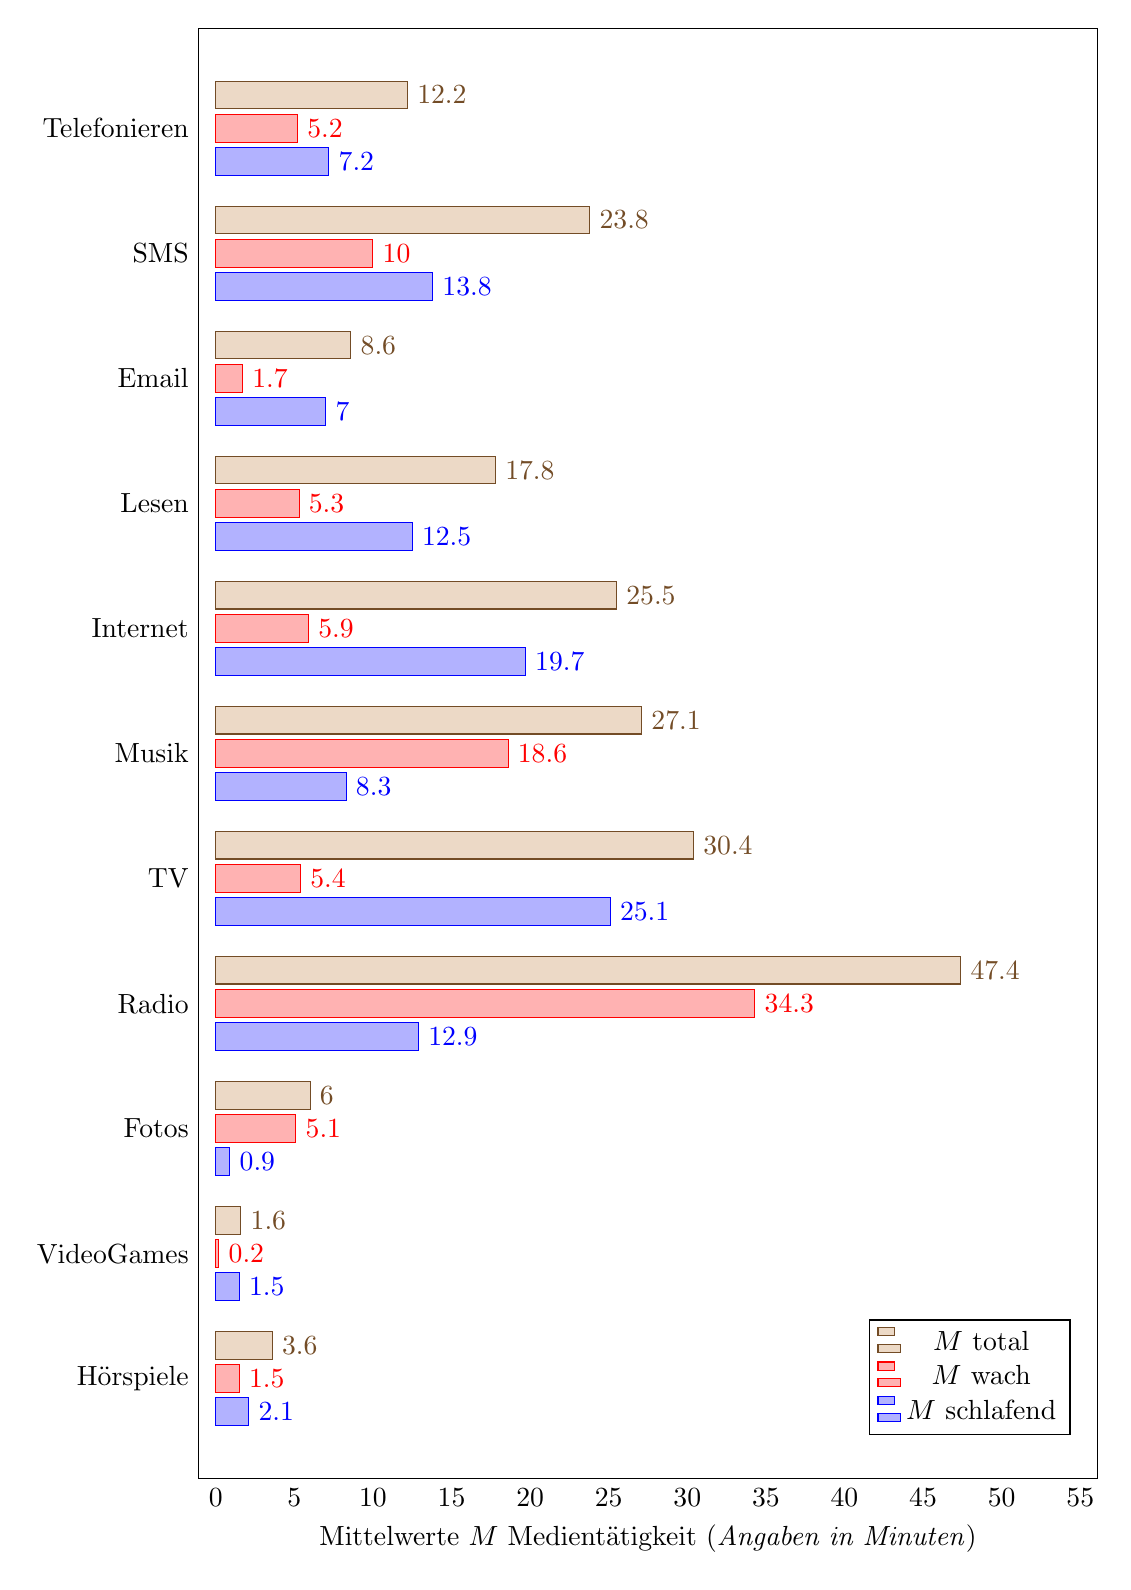
\begin{tikzpicture}[scale=1]
  \begin{axis}[
    xbar,
    %y axis line style = { opacity = 0 },
    %axis x line       = none,
    tickwidth         = 0pt,
    xmin              = 0,
    xmax              = 55,
    enlarge y limits  = 0.08,
    enlarge x limits  = 0.02,
    reverse legend,
    legend pos=south east,
    ytick             = data,
    xlabel            = {Mittelwerte $M$ Medientätigkeit (\textit{Angaben in Minuten})},
    height            = 20cm,
    width             = 13cm,
    symbolic y coords = {Hörspiele, VideoGames, Fotos, Radio, TV, Musik, Internet, Lesen, Email, SMS, Telefonieren},
    nodes near coords,
    nodes near coords align={horizontal},
  ]
  %geschlafen
  \addplot coordinates { (7.2,Telefonieren)(13.8,SMS)(7,Email)(12.5,Lesen)(19.7,Internet)(8.3,Musik)(25.1,TV)(12.9,Radio)(0.9,Fotos)(1.5,VideoGames)(2.1,Hörspiele)};
  %wach
  \addplot coordinates { (5.2,Telefonieren)(10,SMS)(1.7,Email)(5.3,Lesen)(5.9,Internet)(18.6,Musik)(5.4,TV)(34.3,Radio)(5.1,Fotos)(.2,VideoGames)(1.5,Hörspiele)};
  %total
  \addplot coordinates { (12.2,Telefonieren)(23.8,SMS)(8.6,Email)(17.8,Lesen)(25.5,Internet)(27.1,Musik)(30.4,TV)(47.4,Radio)(6,Fotos)(1.6,VideoGames)(3.6,Hörspiele)};
  
  \legend{\text{$M$ schlafend}, \text{$M$ wach},  \text{$M$ total}}
  \end{axis}
\end{tikzpicture}
\end{figure}

\begin{figure}%[htp]
\caption{Anzahl Geräte im Haushalt}\label{fig:AppGeräteHaushalt}
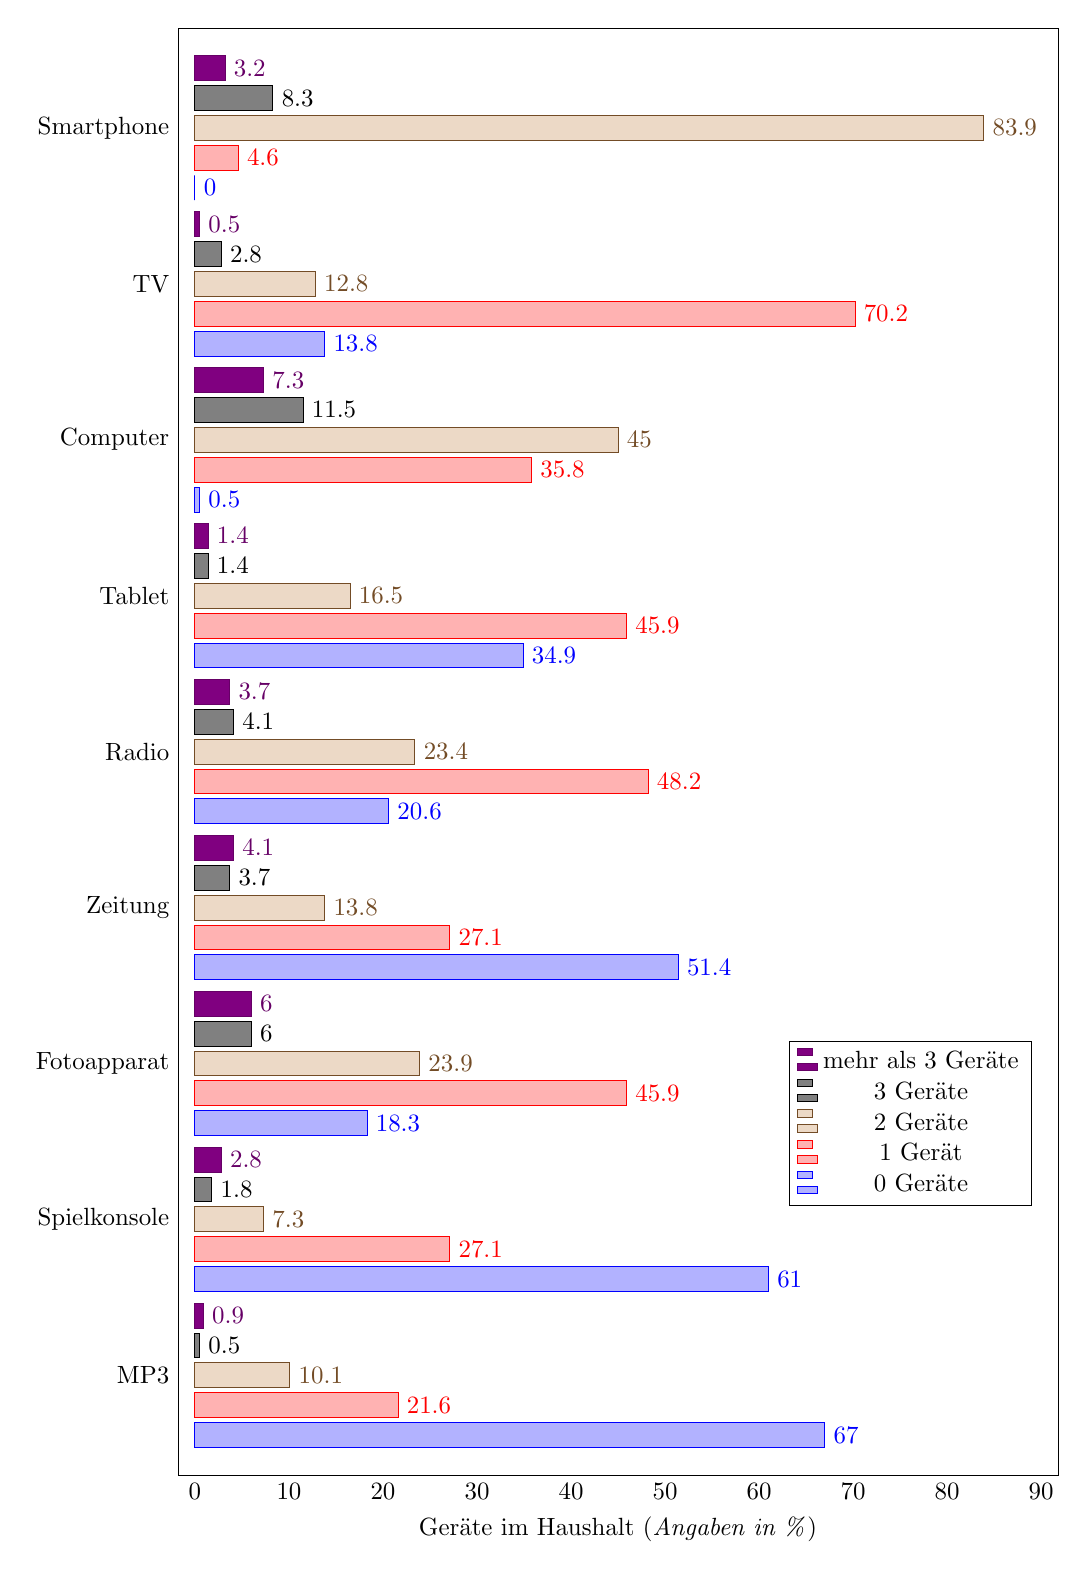
\begin{tikzpicture}[scale=.9]
  \begin{axis}[
    xbar ,
    %y axis line style = { opacity = 0 },
    %axis x line       = none,
    tickwidth         = 0pt,
    xmin              = 0,
    xmax              = 90,
    enlarge y limits  = 0.08,
    enlarge x limits  = 0.02,
    %legend pos=south east,
    legend style={at={(0.97,0.3)}},
    reverse legend,
    ytick             = data,
    xlabel            = {Geräte im Haushalt (\textit{Angaben in \%})},
    height            = 22cm,
    width             = 14cm,
    symbolic y coords = {MP3, Spielkonsole, Fotoapparat, Zeitung, Radio, Tablet, Computer, TV, Smartphone},
    nodes near coords,
    nodes near coords align={horizontal},
  ]
  %0 Geräte
  \addplot coordinates { (0,Smartphone)(13.8,TV)(.5,Computer)(34.9,Tablet)(20.6,Radio)(51.4,Zeitung)(18.3,Fotoapparat)(61,Spielkonsole)(67,MP3)};
  
  %1 Gerät
  \addplot coordinates { (4.6,Smartphone)(70.2,TV)(35.8,Computer)(45.9,Tablet)(48.2,Radio)(27.1,Zeitung)(45.9,Fotoapparat)(27.1,Spielkonsole)(21.6,MP3)};
  
  %2 Geräte
  \addplot coordinates { (83.9,Smartphone)(12.8,TV)(45,Computer)(16.5,Tablet)(23.4,Radio)(13.8,Zeitung)(23.9,Fotoapparat)(7.3,Spielkonsole)(10.1,MP3)};
  
  %3 Geräte
  \addplot coordinates { (8.3,Smartphone)(2.8,TV)(11.5,Computer)(1.4,Tablet)(4.1,Radio)(3.7,Zeitung)(6,Fotoapparat)(1.8,Spielkonsole)(.5,MP3)};
  
  %>3 Geräte
  \addplot coordinates { (3.2,Smartphone)(.5,TV)(7.3,Computer)(1.4,Tablet)(3.7,Radio)(4.1,Zeitung)(6,Fotoapparat)(2.8,Spielkonsole)(.9,MP3)};
  
  \legend{\text{0 Geräte}, \text{1 Gerät}, \text{2 Geräte}, \text{3 Geräte}, \text{mehr als 3 Geräte}}
  \end{axis}
\end{tikzpicture}
\end{figure}

\begin{figure}[htp]
\caption{Medienverzicht}\label{fig:AppMedienverzicht}
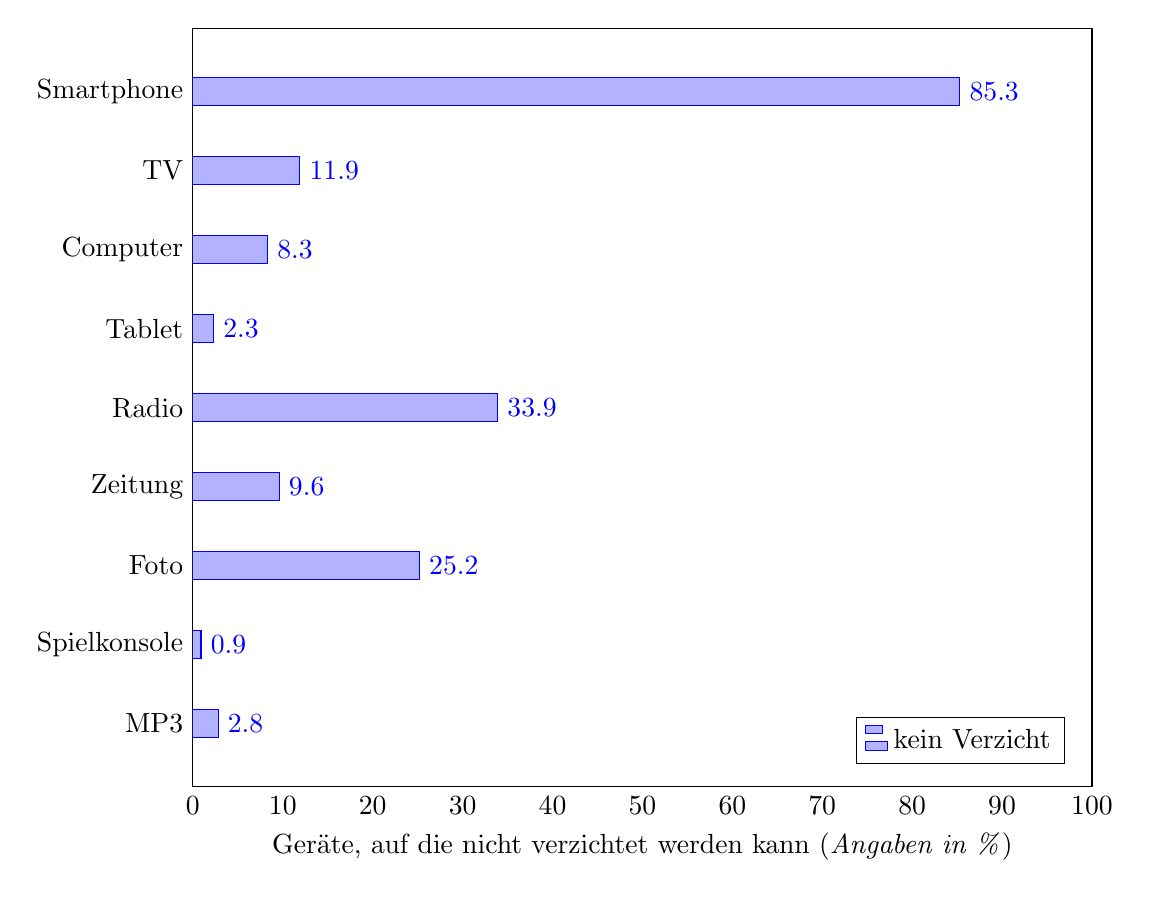
\begin{tikzpicture}[scale=1]
  \begin{axis}[
    xbar,
    %y axis line style = { opacity = 0 },
    %axis x line       = none,
    tickwidth         = 0pt,
    xmin              = 0,
    xmax              = 100,
    %enlarge y limits  = 0.1,
    %enlarge x limits  = 0.02,
    reverse legend,
    legend pos=south east,
    ytick             = data,
    xlabel            = {Geräte, auf die nicht verzichtet werden kann (\textit{Angaben in \%})},
    %height            = 20cm,
    width             = 13cm,
    symbolic y coords = {MP3, Spielkonsole, Foto, Zeitung, Radio, Tablet, Computer, TV, Smartphone},
    nodes near coords,
    nodes near coords align={horizontal},
  ]
  %nicht verzichten
  \addplot coordinates { (85.3,Smartphone)(11.9,TV)(8.3,Computer)(2.3,Tablet)(33.9,Radio)(9.6,Zeitung)(25.2,Foto)(.9,Spielkonsole)(2.8,MP3)};
  
  \legend{kein Verzicht}
  \end{axis}
\end{tikzpicture}
\end{figure}
